\subsection{Implementation of system components}

In the previous section we have described requirements on the individual system components. In following paragraphs we explain, how the prototype was implemented, following the requirements listed earlier. We elaborate on how the development was approached and what technologies were used, for every individual system component. 
% 
% 
% 
%       __   __  
%  /\  |__) |__) 
% /~~\ |    |    
%&&&&&&&&&&&&&&&&&&&&&&&&&&&&&&&&&&&&&&&&&&&&&&&&&&&&&&&&&&&&&&&&&&&&&&&&&&&&&&&&&&&&&&&&&&&&&&
% 
\subsubsection{Application front end} 
To implement the functional requirements mentioned in section~\ref{sec:app-front-reqs} (page \pageref{sec:app-front-reqs}), we choose the Android platform. Currently, it is the most used operating system in the world\footnotemark which ensures compatibility with significant number of devices. It is capable of carrying out the tasks outlined above and it does not require a centralised server to operate (as opposed to a website/web application). Development tools and documentation available free of charge and author's previous knowledge of Android programming were the further supporting arguments for Android. Android \acrshort{api} version 26 (Android Oreo) was chosen, as it is the newest supported version at the time of writing, although this has little practical implications. The prototype uses some user-interface features that were first introduced in \acrshort{api} version 22, so the minimal required Android version could be rolled back to this version without any changes.
% 
\footnotetext{\url{http://gs.statcounter.com/os-market-share}, as of 06-05-2018. See //REFERENCE TO APPENDIX for details}

In conjunction with Android, standard Java programming language was used. This is as opposed to Kotlin, a statically typed programming language, which was developed by JetBrains\footnotemark and pronounced the official Android programming language by Google on 17th May 2017~\cite{Vasic2017MasteringKotlin}. 
% 
\footnotetext{JetBrains is a company that created IntelliJ and other popular \acrshort{ide}s. \url{https://www.jetbrains.com/}}
% 
Many industry professionals suggest migrating to Kotlin as it offers several advantages~\cite{Vasic2017MasteringKotlin} \footnotemark, but it has no direct implication on the prototype, as it compiles to the same byte-code as Java.
% 
\footnotetext{\url{https://medium.com/@magnus.chatt/why-you-should-totally-switch-to-kotlin-c7bbde9e10d5}, accessed 06-05-2018}

We describe the structure of the prototype using the terminology of the \acrfull{modelvp} architecture pattern, which describe the architecture of an application in three layers or interfaces:
\begin{enumerate*}[label=(\roman*)]
    \item \textit{Model}
    \item \textit{View} and
    \item \textit{Presenter}
\end{enumerate*}.
The prototype does not fully succeed in following this patter, but it does share the major features with it. In the prototype, the split between model and presenter is not ideal and these two layers partially overlap. The approximation is as follows:
\begin{itemize}[noitemsep]
    \item Fragments have the role of the \textit{view} part
    \item \texttt{MainActivity} and wrapper classes have the role of the \textit{presenter} part
    \item \texttt{TradeDeal} and \texttt{BtcOffer} have the role of the \textit{model}.
\end{itemize}

\paragraph{View} The view part of the \acrshort{modelvp} is represented by eight fragment classes. Each fragment represents one screen of the application. XML files are used to describe the user interface elements of each fragment. Fragments read user inputs from these elements and update them accordingly with information received from \textit{presenter} interface. Example of such fragment is \texttt{DeployContractFragment}, which displays wallet balance in one \texttt{TextView} and reads user's input from another.

\paragraph{Presenter} 
\begin{sloppypar}
To navigate between fragments and update the view with new data, \texttt{MainActivity} is used. It implements interface \texttt{OnFragmentInteractionListener} that listens for user interaction in the fragments and responds accordingly. For example if the user selects to create a new offer by clicking on appropriate button, fragment calls the \texttt{onFragmentInteraction} method of \texttt{OnFragmentInteractionListener}, which is implemented in the activity class. \texttt{MainActivity} then initiates fragment transaction and replaces the old fragment with \texttt{CreateOfferFragment}.

The \textit{presenter} part of \acrshort{modelvp} is further complemented by three wrapper classes (\texttt{EthereumWrapper}, \texttt{BitcoinWrapper} and \texttt{FirebaseWrapper}). These classes contain methods to convert data to and from user-comprehensible format (e.g. method \texttt{satoshiToBtcString} from \texttt{BitcoinWrapper} class that converts the amount in Satoshi to more user-friendly format -- decimal Bitcoins) and to communicate with the network (e.g. method \texttt{fetchExistingOffers} in \texttt{FirebaseWrapper} to get data from the database or method \texttt{sendContract} in \texttt{EthereumWrapper} to deploy contract to the network).
\end{sloppypar}

\paragraph{Model}
The \textit{model} interface in the prototype is represented by classes \texttt{BtcOffer} and \texttt{TradaDeal}. The first is used to contain all details of an offer to sell Bitcoins, both when a new offer is created and when existing offers are loaded from the database. When a user decides to proceed with an offer, \texttt{BtcOffer} is transformed into a \texttt{TradeDeal}. Trade deal holds further details of the offer, such as the deploying address and is used during the transaction validation process and during contract deployment.

The Java representation of the smart contract, \texttt{SmartExchange2} is also part of the model. It does not operate any logic in the Android application, but it holds the binary representation of the compiled Solidity code. The methods of this Java representation would also be used to communicate with an already deployed smart contract, although this functionality is currently not implemented in the prototype as it is not needed. \texttt{SmartExchange2} also contains the constructor used to pass initial value to the contract upon deployment. It is important to note, that \texttt{SmartExchange2} is an auto-generated code by the Web3j library, which takes ABI and BIN files of a compiled contract as the input and returns a single Java class as the output.

A screenshot of the application is shown in Figure \ref{fig:app-screenshot}.

\begin{figure}[ht]
    \centering
    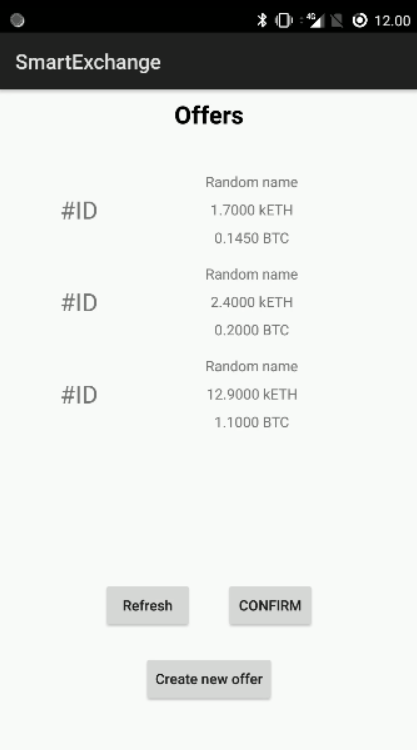
\includegraphics[height=.4\textheight]{screenshots/screen010}
    \caption{Screenshot of the first application screen. It whows three Bitcoin offers, which were loaded from the database.}
    \label{fig:app-screenshot}
\end{figure}
% 
% 
% 
%       __   __   ___ 
% |\ | /  \ |  \ |__  
% | \| \__/ |__/ |___
%&&&&&&&&&&&&&&&&&&&&&&
% 
\subsubsection{Node}
As mentioned in the State of the Art \pageref{sec:eth-clients}, there are multiple Ethereum clients that can be used to deploy transactions to the network. Etherumj could be used to connect the front end application to the Ethereum network, functioning as a full network node. However, running a full node on the Android platform is not a viable solution, due to limitations of mobile devices. These limitations include storage, network bandwidth and power consumption\footnotemark.%
\footnotetext{Proof-of-concept solutions offering a full node deployment on the Android platform exist for the Bitcoin protocol, but they maintain storage capacity and network connectivity as the limitations and are not widely used in practice. \url{https://github.com/greenaddress/abcore\#limitations}, accessed 18-05-2018}
% 
Fully connected node maintains a local copy of the blockchain (storage) and regularly communicates with the network peers to get the most recent block (network and battery consumption). Alternative solution to lower the load on the mobile device would be to run a light client\footnotemark, which is targeted specifically for mobile devices and that does not maintain a local copy of the whole blockchain.
% 
\footnotetext{\url{https://github.com/ethereum/wiki/wiki/Light-client-protocol}, accessed 17-05-2018}

To speed up the development, we decided to use a remotely hosted node for this prototype. Instead of deploying own remote Ethereum node, a node-hosting service Infura was chosen. Upon creating an account on Infura’s website, developer is presented with a series of API endpoints – one endpoint for all major Ethereum networks (Mainnet, Kovan, Rynkeby…). Endpoints accept connections from any client and no authentication is needed. This is not an issue, since by design, the prototype signs the transaction on device, before it is deployed to the network. The node therefore only processes singed transactions and does not have access to users' private keys.

% 
%  __              __  ___     __   __       ___  __        __  ___ 
% /__`  |\/|  /\  |__)  |     /  ` /  \ |\ |  |  |__)  /\  /  `  |  
% .__/  |  | /~~\ |  \  |     \__, \__/ | \|  |  |  \ /~~\ \__,  | 
%&&&&&&&&&&&&&&&&&&&&&&&&&&&&&&&&&&&&&&&&&&&&&&&&&&&&&&&&&&&&&&&&&&&&
% 
\subsubsection{Smart Contract}
The contract is written in the Solidity language, as it is currently the most popular language for smart contracts and offers simple JavaScript-like syntax~\cite{Tikhomirov2018Ethereum:Perspectives}. The version of Solidity does not have crucial role to the functionality of the Smart Contract, so we decided to use the latest version available (0.4.21)\footnotemark. The Smart Contract was written using Remix, an in-browser \acrshort{ide}, which enables sandbox contract testing. Oraclize (//EXPLAIN WTH IS ORACLIZE) version of Remix was also used to test the functionality of an oracle.
% 
\footnotetext{One implication of using version of Solidity above 0.4.0 is that a special keyword \texttt{emit} needs to be used to indicate an event in the code.}

Smart contract\footnotemark in Solidity was then compiled into \texttt{BIN} (binary) and \texttt{ABI} files, using the \textit{solc} compiler.
% 
\footnotetext{The code of the smart contract can be seen in Appendix~\ref{sec:appendix-code} on page \pageref{sec:appendix-code} and also in the attached code}
% 
The \texttt{BIN} file contains the Solidity code compiled into Ethereum Virtual Machine bytecode and \texttt{ABI} (Application Binary Interface) file contains information about how to interact with the Smart Contract. Encoding of the \texttt{ABI} file is part of the Ethereum protocol specification\footnotemark. These \texttt{BIN} and \texttt{ABI} files where then used by Web3j command line tools to generate Java representation of the Smart contract\footnotemark.
% 
\footnotetext{The wrapper class can be found under the name \texttt{SmartExchange2.java} among the applicaiton source files.}
% 
Web3j command line tools are an extension of the Web3j library, used to automate the creation of Java file representing the Smart Contract. On top of the compiled smart contract in binary form, this Java file also includes wrapper methods to invoke the custom constructor and the methods of the contract.
% 
\footnotetext{\url{https://solidity.readthedocs.io/en/develop/abi-spec.html}, accessed 17-05-2018}
% 
% 
%   __   __        __        ___ 
%  /  \ |__)  /\  /  ` |    |__  
%  \__/ |  \ /~~\ \__, |___ |___ 
%&&&&&&&&&&&&&&&&&&&&&&&&&&&&&&&&&&&&
% 
\subsubsection{Oracle}
As noted in Section \ref{sec:data-input} (p. \pageref{sec:data-input}), there are currently not many providers that offer oracle services. For the prototype there were two alternatives: implementing an own oracle or using an off-the-shelf service. We decided to go with the latter, since implementing an oracle is a complex task and it was not the focus of this project. We chose to implement the Oraclize service, as it is currently the widely used in the community and inlcudes extensive documentation and testing environment.

To implement Oraclize in a project, the smart contract must import and extend \texttt{usingOraclize} class, which is provided by Oraclize. Extending this class allows the developer to directly call \texttt{oraclize\_query} method that manages creating a query that can be understood by Oraclize servers. This method takes at least two arguments: a data source and an argument for the data source. Currently supported data sources include providers like WolframAlpha%
\footnote{WolframAlpha is a computational knowledge engine that includes extensive collection of data, algorithms and methods. \url{http://www.wolframalpha.com/about.html}, accessed 17-05-2018}%
and \acrshort{ipfs}%
\footnote{\acrfull{ipfs} is a peer-to-peer protocol that connects all participating devices with the same system of files. \url{https://github.com/ipfs/ipfs}, accessed 17-05-2018},%
together with a \textit{random} option and an option to send a query to a URL address. Another optional argument is time delay in seconds. By default, Oraclize responds to a query right away. If the delay argument is present, Oraclize will wait for specified amount of time before issuing a reply.

For the smart contract to register a reply from Oraclize, it must implement a \texttt{\_\_callback} method, which will be called by an Oraclize-issued smart contact together with the result. It is in this method that the smart contract needs to handle the response.
%
% 
%  __        __   __        __                   
% |__) |    /  \ /  ` |__/ /  ` |__|  /\  | |\ | 
% |__) |___ \__/ \__, |  \ \__, |  | /~~\ | | \|
%&&&&&&&&&&&&&&&&&&&&&&&&&&&&&&&&&&&&&&&&&&&&&&&&&
% 
\subsubsection{Blockchain explorer}
Most of the blockchain explorer providers available today have would be capable of supporting our system. Many have a defined API and most of these APIs can provide information about the balance of an address. Different providers require different format of the API query and their answers have different formatting. Since the response to the query needs to be processed by the smart contract, a simpler response that does not require extensive processing would be preferred.

\begin{sloppypar}
Examples given in State of the Art (//LINK TO SECITON) were considered as candidates. The simplest API is the \textit{Simple Query API} provided by the Blockchain.info platform. A request query to this API is a simple HTTP GET method to \texttt{https://blockchain.info/q/getreceivedbyaddress/X}, where \texttt{X} is substituted with the requested Bitcoin address. A response from this API is a HTTP OK response containing a single number -- the balance of the address in Satoshi. Blockchain.info also allows to filter out unconfirmed transactions out of the address balance. This is done by attaching \texttt{?confirmations=Y} to the end of the request endpoint, where Y is substituted with the number of desired confirmations, before a transaction is considered for the address balance. The implementation of Blockchain.info satisfies the functional requirement BE-FR-1 specified in Table~\ref{tab:reqs-block-explorer} (page \pageref{tab:reqs-block-explorer}).
\end{sloppypar}
% 
% 
%  __   __                           __       ___    __       
% /  ` /  \  |\/|  |\/| |  | |\ | | /  `  /\   |  | /  \ |\ | 
% \__, \__/  |  |  |  | \__/ | \| | \__, /~~\  |  | \__/ | \|
%&&&&&&&&&&&&&&&&&&&&&&&&&&&&&&&&&&&&&&&&&&&&&&&&&&&&&&&&&&&&&
% 
\subsubsection{Communication back end}
The data processed by communication back end consists of users' Bitcoin and Ether offers. The amount of data in the database is proportional to the number of users, since most people only carry out one transaction at the time. Furthermore, the database does not need to maintain a history of executed transactions (since the transaction history is well captured in the Bitcoin and Ethereum blockchains), therefore we can assume that the database does not need to handle more then couple of hundreds individual offers at once. This simplifies the selection of the database, since this is relatively low database load. Furthermore, as noted in the requirement section, users may still be able to agree on transaction terms via another platform outside our system, so even if the back end is not operational, the system can still be used. 

Database structure is not crucial factor for the database implementation. Each offer comprises the same type of data -- a single offer to buy Ether includes following details:
\begin{itemize}[noitemsep]
    \item Amount of Bitcoins offered
    \item Amount of Ether requested
    \item Destination Ethereum address (where the Ether will go after the transaction)
    \item Nickname of the user who created the offer (optional)
\end{itemize}

Offers for buying Bitcoin have the same pattern, but Bitcoin and Ether are exchanged and \textit{Destination Ethereum address} is replaced by \textit{Destination Bitcoin address}. The regular structure in the data indicates that an SQL database may be better fit to handle the data, on the other hand, noSQL allows for the structure to be changed easily, shall such need arise~\cite{Xplenty2017TheMedium}.

For the back end platform, we decided to use Firebase, which is a noSQL database storing data in JSON format. This decision was motivated by the fact that Firebase can be easily integrated with an Android application and offers interface to push real-time date updates into the Android application. Besides storing users' offers, the back end also serves as the coordination channel for the users. We use the \texttt{offerStatus} field to indicate the progress of the transaction to primary and secondary user. Series of prompts presented to the users in the front end application changes the status of this field and enables the users to proceed with the transaction. Let us consider that the secondary user created an offer to sell Bitcoins and buy Ether. The status codes associated with this offer would be as shown in Table~\ref{tab:offer-status}. When a user performs an action in the application that advances the progress of the transaction, the \texttt{offerStatus} field in the database is updated. Firebase will detect this change and push this update to the front end application of user's trading partner.

\begin{table}[ht]
    \centering
    \begin{tabularx}{\textwidth}{|l|l|X|}
        \hline
        \textbf{Offer Status}&\textbf{Code}&\textbf{Description}\\
        \hline
        \hline
        \texttt{DATA\_STATUS\_NEW}&11&New offer was created by the Secondary user and sent to the database\\
        \hline
        \texttt{DATA\_STATUS\_THEY\_CONFIRMED}&12&Primary user indicated their interest in this offer\\
        \hline
        \texttt{DATA\_STATUS\_YOU\_CONFIRMED}&13&Secondary user confirmed that they wish to engage in a transaction\\
        \hline
        \texttt{DATA\_STATUS\_ACCEPTED }&14&Primary user deployed the Smart contract to the network\\
        \hline
    \end{tabularx}
    \caption{Status codes associated with a Bitcoin offer. Certain user actions trigger the change of the offer status.}
    \label{tab:offer-status}
\end{table}